    z = [0 1 1.01 2 2.01 3 3.01 4 4.01 5 5.01 6];

    % Cummulative
    Fz = [0 0 .06 .06 .29 .29 .64 .64 .91 .91 1 1];

    % Lay mau ngau nhien
    sample = randsrc(1,N,[Z; PZ]); % tuy chon so luong mau N ra vi tri xac suat 
    [nz,cz] = hist(sample,n); % phan lam n hop 
    % Tan suat
    fz = nz/N;
    CDFz = cumsum(fz);

    % Tinh toan kiem dinh Pearson
    % Cac tan so ly thuet
    Ei =  PZ*N;

    % Tieu chuan kiem dinh
    chi_P = sum( ((nz - Ei).^2) ./ Ei );

    % Tra gia tri toi han
    chi_J = chi2inv(.95, n - 1);

    subplot(1,2,1)
    % Bieu dien pdf
    plot(Z, PZ, 'r','LineWidth',2)
    hold on

    % 
    bar(cz, fz, 'b')
    hold on
    axis([0 6 0 0.5]) % xac dinh bien do ve

    subplot(1,2,2)
    % Bieu dien CDF Fz
    plot(z,Fz,'r','LineWidth',2) % CDF cua mo hinh
    hold on
    plot(cz,CDFz,'b','LineWidth',1) % CDF cua mo hinh CDFz
    hold off
    axis([0 6 0 1.2]) % xac dinh bien do ve
    figure(1)
end

\end{lstlisting}
\end{lstlisting}

\begin{figure}[h!]
    \centering
    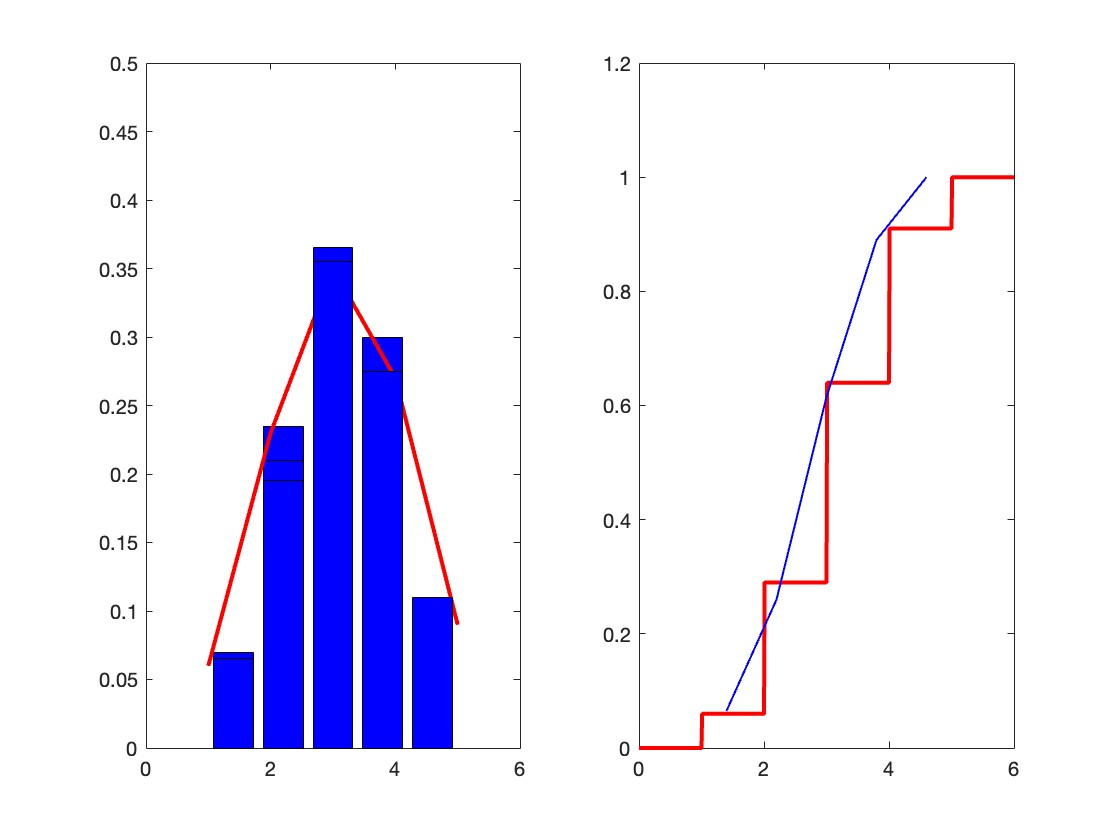
\includegraphics[width=1\linewidth]{../../assets/images/main-content-image.jpg}
    \caption{Hình minh họa 1}
    \label{fig:image1-matlab}
\end{figure}

\begin{lstlisting}[language=Matlab]
    \begin{lstlisting}
function Ngocppmohinh(c,j1,j2)
    %UNTITLED Summary of this function goes here
    % Version: 1.0
    %  Date: 10/09/24

    % So tham so
    numpara=j2-j1+1;
    % Dat cac tham so ban dau
    xmin=0; xmax=20; ymin=0; ymax=numpara*4;

    % Import the data
    singletons = readtable("singletons.xlsx");

    % Ve cac doi tuong thanh phan

    for i=1:numpara
    % Ve cac nut tren
    plot((xmin+xmax)/2,ymax-4*(i-1),'ob');
    hold on
    % Ve cac vi tri trang thai
        % tim vi tri cac hang trang thai cua tham so i
        hi=find([singletons{:,2}]==j1+i-1);
        % so trang thai thu i
        ni=length(hi);
        % so gia chia deu chieu ngang x
        dx=(xmax-xmin)/(ni+1);
        % vecto cac diem chia deu chieu ngang x
        x=xmin:dx:xmax;
        % Ve cac duong che ra
        % Vong lap cho tung trang thai
        for t=1:ni
        % Ve cac duong che ra
        plot([x(t+1) (xmin+xmax)/2],[ymax-4*(i-1)-2 ymax-4*(i-1)],'-r');
        hold on
        % Ve cac nut
        plot(x(t+1),ymax-4*(i-1)-2,'ob');
        hold on
        % Chen cac ten trang thai
        text(x(t+1)+.4,ymax-4*(i-1)-2-.4,singletons{hi(t),1});
        % Chen cac duong hoi tu
        plot([x(t+1) (xmin+xmax)/2],[ymax-4*(i-1)-2 ymax-4*(i-1)-4],'-r');
        hold on
        % Chen xac suat
        text(x(t+1)-.9, ymax-4*(i-1)-2+.4, [num2str(singletons{hi(t),5})]);
        end % t=1:ni
    end % for i=1:numpara
